\documentclass{beamer}
\usepackage{algorithm}
\usepackage{algpseudocode}
\usepackage{caption}
\usepackage{hyperref}
\usepackage{booktabs}
\renewcommand\vec[1]{\ifstrequal{#1}{0}{\ensuremath{\mathbf{0}}}{\ensuremath{\boldsymbol{#1}}}}
\setbeamertemplate{headline}{}


\usetheme[compress]{Berlin}
\setbeamertemplate{page number in head/foot}[framenumber]
\captionsetup{justification=centering, font={scriptsize}, skip=0pt}

\title[Medios Granulares y Dinámica Peatonal]{Medios Granulares y Dinámica Peatonal: Trabajo Práctico N°5}
\subtitle{72.25 - Simulación de Sistemas}
\author[M. Barnatán, I. Maruottolo Quiroga, I. Pedemonte Berthoud]{
  Martín Alejandro Barnatán\inst{1} \and 
  Ignacio Martín Maruottolo Quiroga\inst{2} \and 
  Ignacio Pedemonte Berthoud\inst{3}
}
\institute[ITBA]{
  \inst{1} mbarnatan@itba.edu.ar (64463) \\
  \inst{2} imaruottoloquiroga@itba.edu.ar (64611) \\
  \inst{3} ipedemonteberthoud@itba.edu.ar (64908) \\
}
\date{2025 2C | Grupo Nº10}
\titlegraphic{\includegraphics[height=1.2cm]{resources/itba.png}}

\makeatletter
\beamer@theme@subsectionfalse
\makeatother

\AtBeginSection[]{
    \begin{frame}
        \begin{beamercolorbox}[sep=8pt,center]{title}
            \usebeamerfont{title}\insertsection
        \end{beamercolorbox}
    \end{frame}
}

\begin{document}

\begin{frame}
  \titlepage
\end{frame}

% Sección 1
\section{Introducción}
\begin{frame}{Sistema Real}
Estudio de un sistema peatonal de N agentes que se mueven en un plano con una velocidad deseada y se evitan mediante una regla de evasión anisotrópica (AA-CPM).
  \begin{columns}[T,onlytextwidth]
    \begin{column}{0.50\textwidth}
    \begin{itemize}
      \item Flujos en corredores.
      \item Interacción con obstáculos.
      \item Cuellos de botella.
    \end{itemize}
    \end{column}
    \hfill
    \begin{column}{0.40\textwidth}
      \centering
      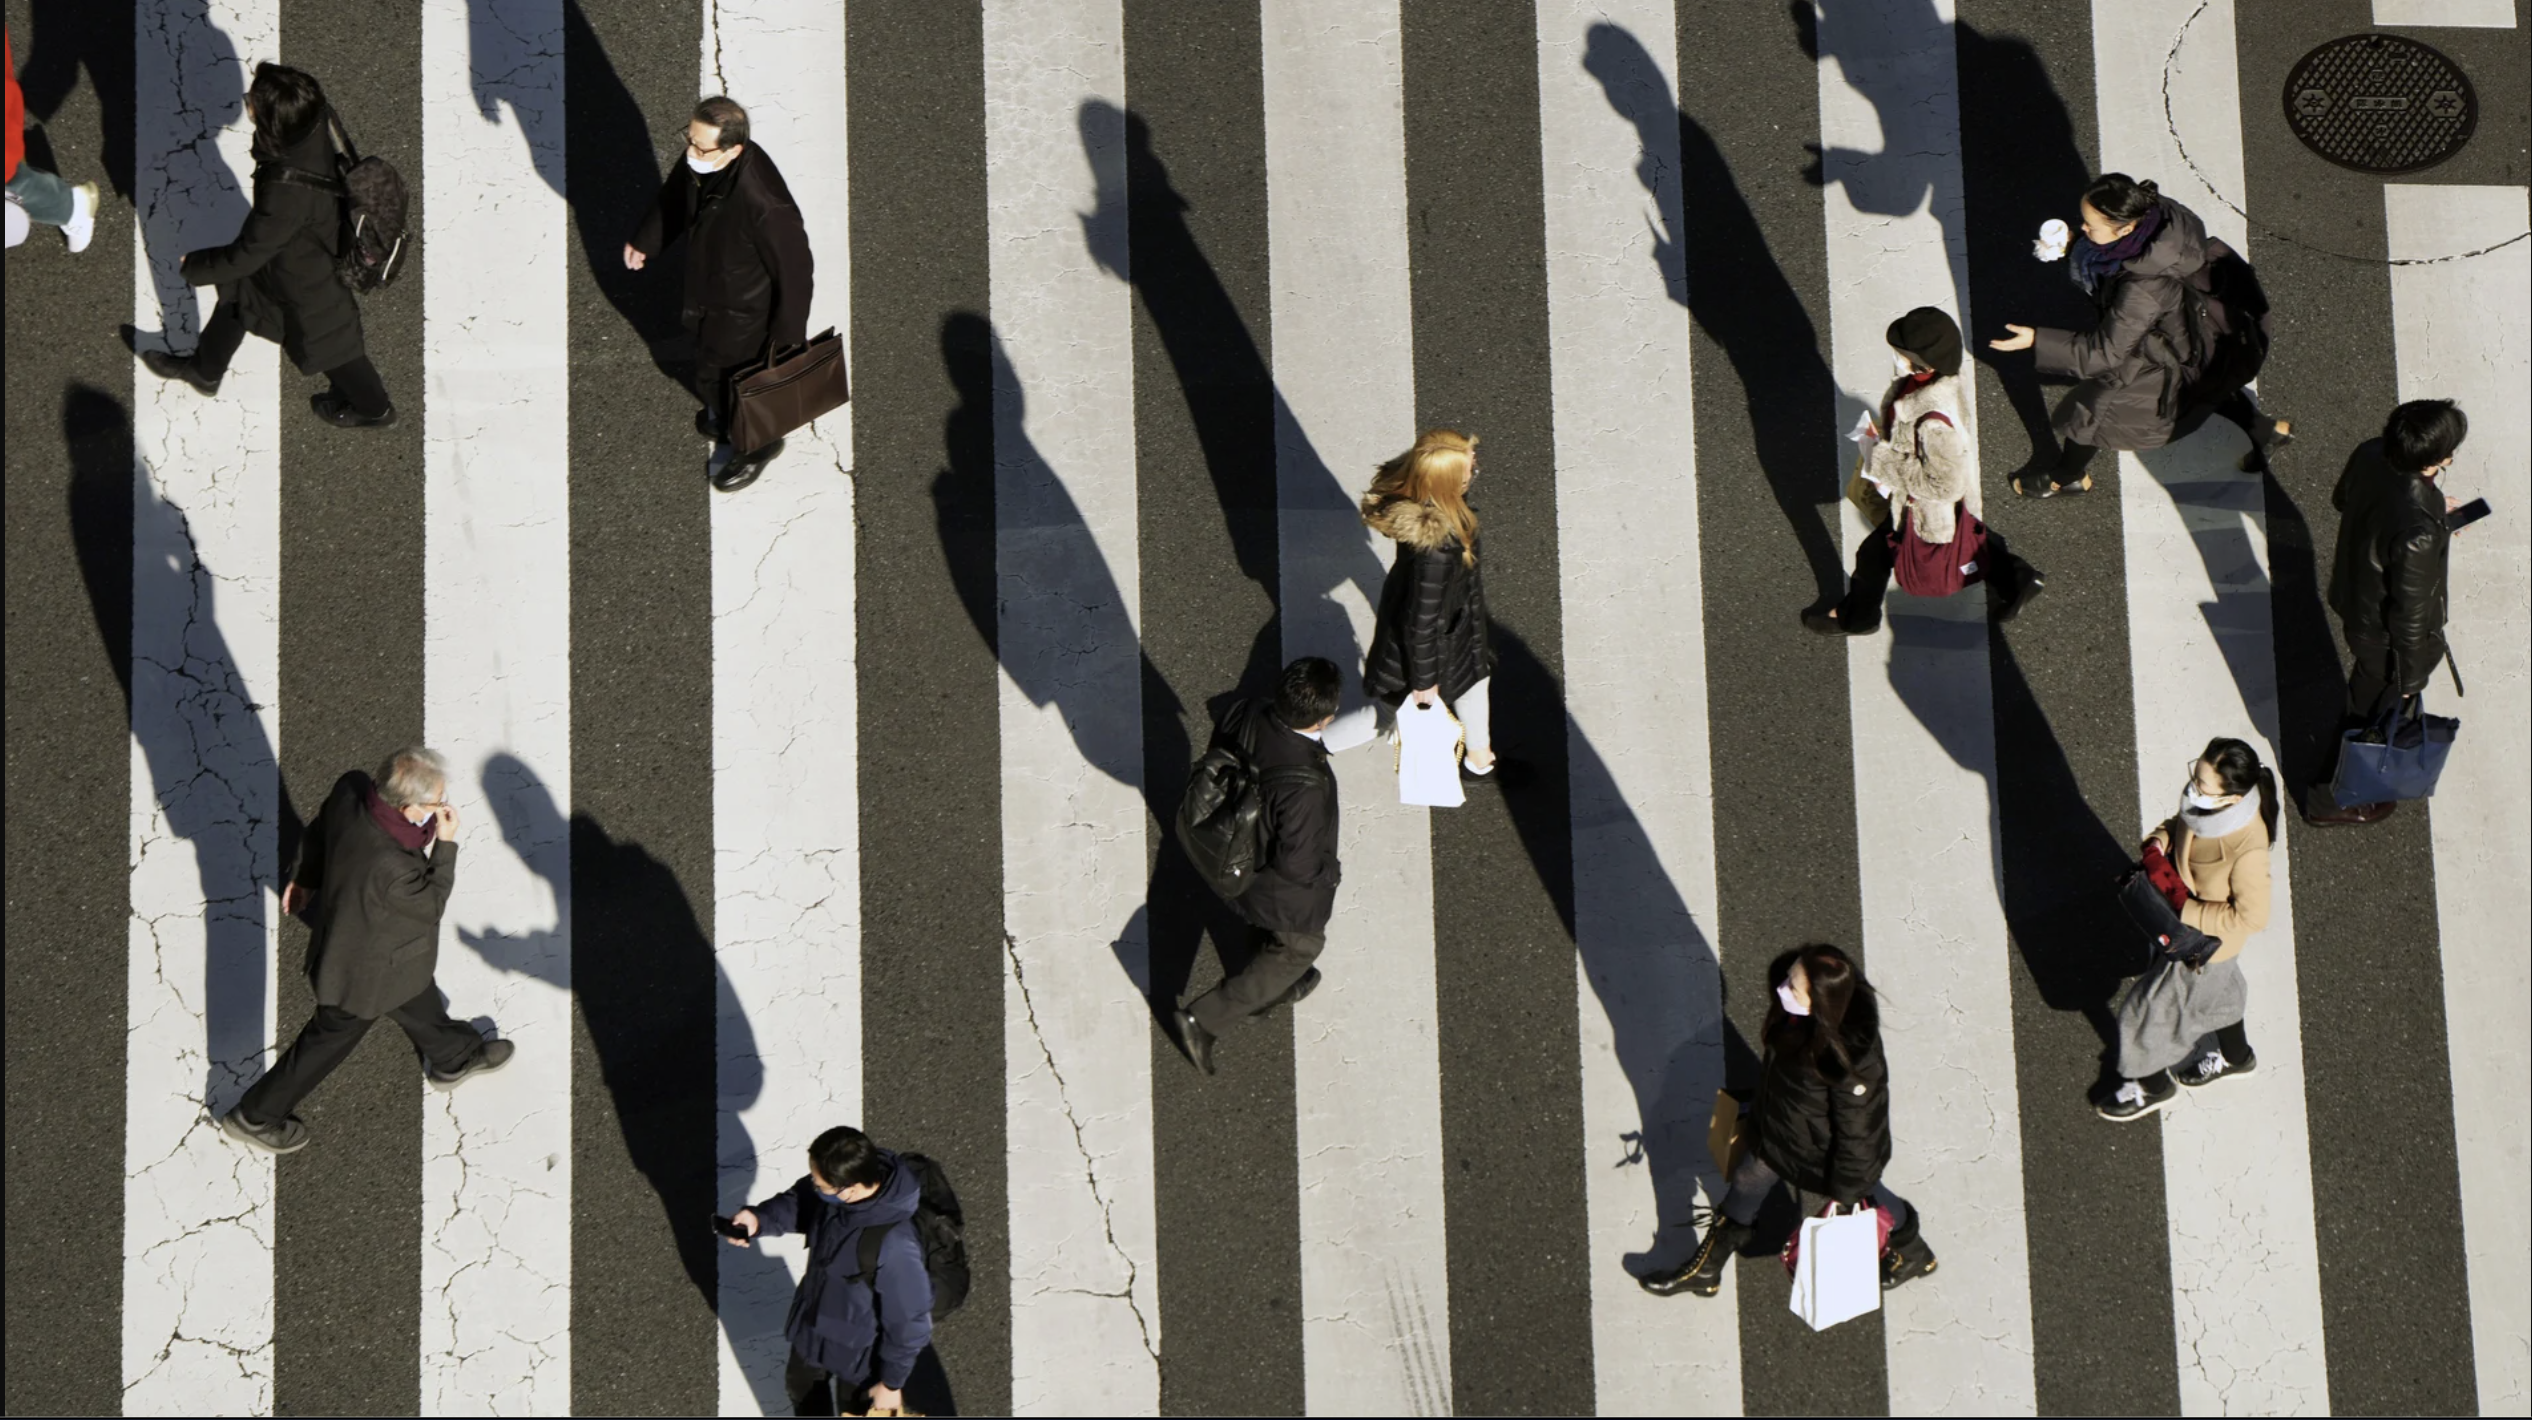
\includegraphics[width=\linewidth]{resources/peatones.png}
    \end{column}
  \end{columns}
\end{frame}

\begin{frame}{Fundamentos}{Esquema del Modelo AA-CPM}
        \begin{columns}[c,onlytextwidth]
        \centering
        \begin{column}{0.50\textwidth}
            \begin{figure}[htbp]
                \centering
                \includegraphics[width=1\textwidth]{resources/paper1.png}
            \end{figure}
        \end{column}
        \hfill
        \begin{column}{0.50\textwidth}
            \begin{figure}[htbp]
                \centering
                \includegraphics[width=1\textwidth]{resources/paper2.png}
            \end{figure}
        \end{column}
      \end{columns}
\end{frame}

\begin{frame}{Fundamentos}{Modelo de Partículas Contráctiles Anisotrópicas con Evasión}
    El radio $r$, la posición $\vec{r}$ y la velocidad $\vec{v}$ se obtienen:
    \begin{equation*}
        r=\left\{
        \begin{array}{ll}
        r_{min} & \text{si la partícula está en colisión},\\
        r(t-\Delta t)+r_{max}\Delta t/\tau & \text{si no y } r(t-\Delta t)+r_{max}\Delta t/\tau < r_{max},\\
        r_{max} & \text{otro caso}
        \end{array}
        \right. 
    \end{equation*}
    \vspace{0.2cm}
    \begin{equation*}
        \vec{r}_i(t)=\vec{r}_i(t-\Delta t) + \vec{v}_i^d(t)\Delta t
    \end{equation*}
    \begin{columns}[c,onlytextwidth]
        \centering
        \begin{column}{0.50\textwidth}
            \begin{equation*}
                \vec{v}_i^d= \left\{
                \begin{array}{ll}
                    v^i\vec{e}^{a} & \text{sin contacto front.}, \\
                    v_{max}^d\vec{e}^{ij} & \text{caso contrario} 
                \end{array}
                \right.
            \end{equation*}
        \end{column}
        \hfill
        \begin{column}{0.50\textwidth}
            \begin{equation*}
                v_i=v_{max}^d(\frac{r_i-r_{min}}{r_{max}-r_{min}})^\beta
            \end{equation*}
        \end{column}
      \end{columns}
\end{frame}

\begin{frame}{Fundamentos}{Dirección de Evasión}
    Para la velocidad, las direcciones de evasión son:
    \begin{columns}[T,onlytextwidth]
        \centering
        \begin{column}{0.40\textwidth}
            \centering
            \begin{equation*}
                \vec{e}^{ij}=\frac{\vec{r}_i-\vec{r}_j}{|\vec{r}_i-\vec{r}_j|}
            \end{equation*}
        \end{column}
        \hfill
        \begin{column}{0.60\textwidth}
          \centering
          \begin{equation*}
            \vec{e}^a=((\sum_{j=1}^{2}\vec{n}_c^j)+\vec{n}_c^w+\vec{e}^t)/|(\sum_{j=1}^{2}\vec{n}_c^j)+\vec{n}_c^w+\vec{e}^t|
          \end{equation*}
        \end{column}
    \end{columns}
    \vspace{0.4cm}
    Donde
    \vspace{0.1cm}
    \begin{equation*}
        \vec{n}_c^j=\vec{e}_c^{ij}A_pexp(-d_{ij}/B_p)    
    \end{equation*}
    \vspace{0.1cm}
    \begin{equation*}
        \vec{e}^t=\frac{\vec{T}_i-\vec{r}_i}{|\vec{T}_i-\vec{r}_i|}
    \end{equation*}
    \vspace{0.1cm}
    \begin{equation*}
        \vec{n}_c^w=\vec{e}^{iw}A_w(-d_{iw}/B_w), \vec{e}^{iw}=\frac{\vec{w}-\vec{r}_i}{|\vec{w}-\vec{r}_i|}
    \end{equation*}
\end{frame}

% Sección 2
\section{Implementación}

\begin{frame}{Diagrama UML}
    \begin{figure}[htbp]
        \centering
        \includegraphics[width=1\textwidth]{resources/diagrama.png}
    \end{figure}
\end{frame}

\begin{frame}{Algoritmo Implementado}
    \begin{figure}[htbp]
        \centering
        \includegraphics[width=0.55\textwidth]{resources/algorithm.png}
    \end{figure}
\end{frame}

% Sección 3
\section{Simulaciones}

\begin{frame}{Sistema Estudiado}
    \centering
    \begin{figure}[htbp]
        \centering
        \includegraphics[width=0.6\textwidth]{resources/system.png}
    \end{figure}
\end{frame}

\begin{frame}{Simulaciones}
    Parámetros de entrada fijos:
    \begin{itemize}
        \item $L=6$m - Lado del dominio cuadrado
        \item $v_d=1.7$m/s - Velocidad deseada
        \item $r_f=0.21$m - Radio de la partícula fija
        \item $r_{min}=0.10$m - Radio mínimo
        \item $r_{max}=0.21$m - Radio máximo
        \item $\Delta t=1/33$s - Paso de discretización temporal
    \end{itemize}
    Parámetros de entrada variables:
    \begin{itemize}
        \item $N\in[10, 500]$ - Cantidad de Partículas
    \end{itemize}
    \vspace{0.4em}
    \begin{center}
        \begin{beamercolorbox}[wd=\linewidth,sep=3pt,center]{block body}
            \small Se realizaron 3 simulaciones por cada valor de $N$.
        \end{beamercolorbox}
    \end{center}
\end{frame}

\begin{frame}{Observables Definidos}
    \begin{itemize}
        \item $N_c(t)$: Contactos únicos acumulados en el tiempo $t$.
        \item $Q$: Scanning rate
        \[
        \begin{aligned}
            Q_i &= 
            \frac{\displaystyle \sum_{k\in Est} (t_k-\bar t_i)\,\big(N_{i,k}-\bar N_i\big)}
                 {\displaystyle \sum_{k\in Est} (t_k-\bar t_i)^2}
        \end{aligned}
        \]
        \item $\alpha$: exponente de cola de los tiempos entre contactos $\tau_i = t_{i+1} - t_i$.
    \end{itemize}
    \vspace{0.2em}
    \makebox[\textwidth]{
      \fcolorbox{black}{white}{
        \parbox{.4\textwidth}{\centering
          \[
            \phi \;=\; \dfrac{\displaystyle\sum_{j=1}^{N} \pi r_j^{2}}{L^{2}}
          \]
        }
      }
    }
\end{frame}

% Sección 4
\section{Resultados}
\begin{frame}{Modelo AA-CPM con $L=6$m y $v_d=1.7$m/s}{Animación para $t_f=60$s}
    \begin{columns}[c,onlytextwidth]
        \begin{column}{0.5\textwidth}
            \centering
            \begin{beamercolorbox}[wd=.78\linewidth,sep=2pt,center]{block body}
                \small $N=10$
            \end{beamercolorbox}
            \par\vspace*{5pt}
            \includegraphics[width=.78\linewidth,keepaspectratio]{resources/aacpm-n10.png}
            {\scriptsize Animación completa en: \url{https://youtube.com/shorts/mS2lQY5Knlg}}
        \end{column}
        \begin{column}{0.5\textwidth}
            \centering
            \begin{beamercolorbox}[wd=.78\linewidth,sep=2pt,center]{block body}
                \small $N=500$
            \end{beamercolorbox}
            \par\vspace*{5pt}
            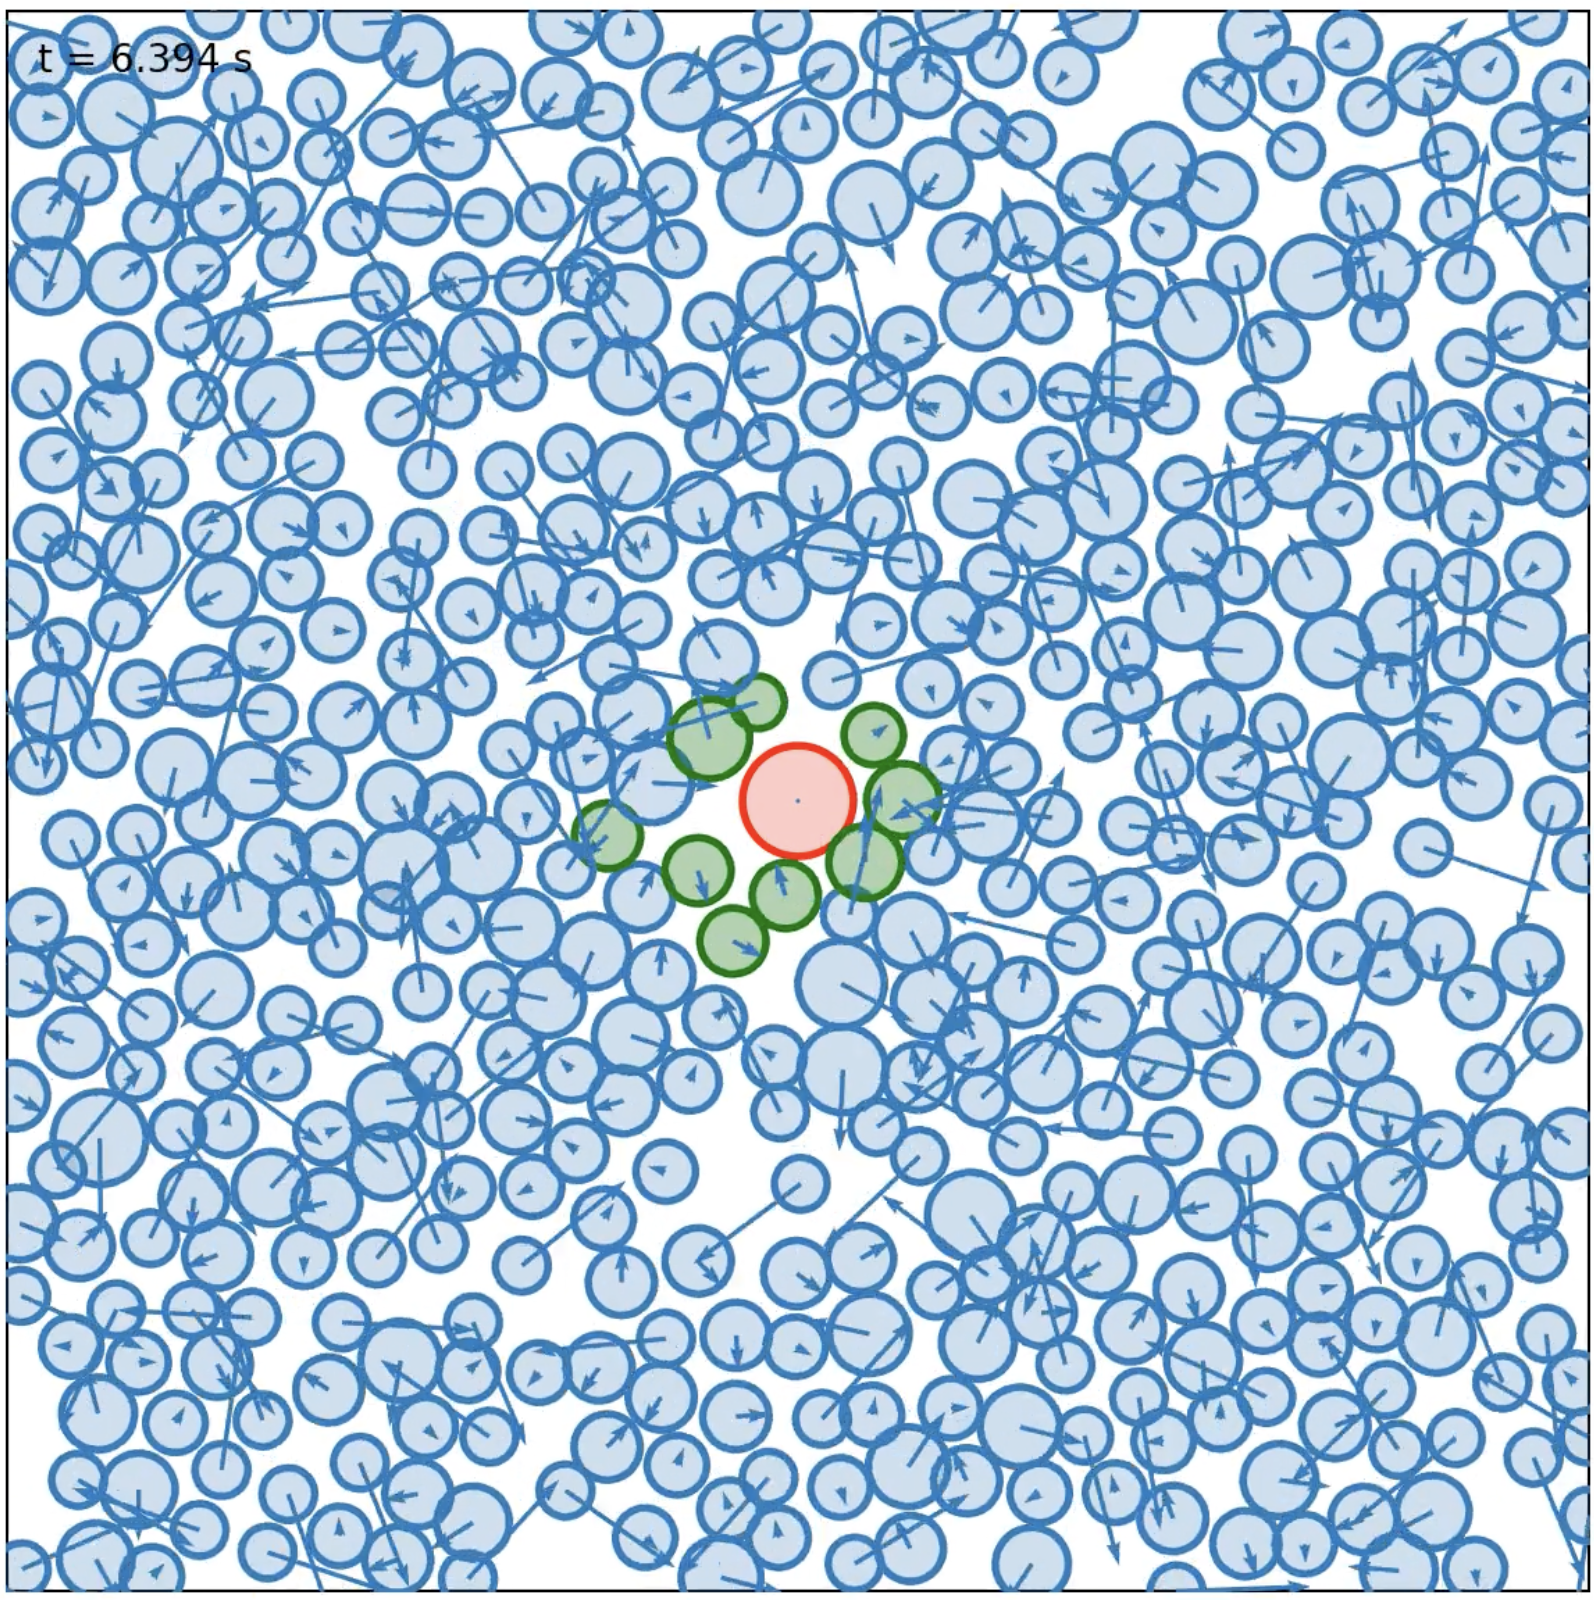
\includegraphics[width=.78\linewidth,keepaspectratio]{resources/aacpm-n500.png}
            {\scriptsize Animación completa en: \url{https://www.youtube.com/shorts/eZaPtlQB8_0}}
        \end{column}
    \end{columns}
\end{frame}

\begin{frame}{Modelo AA-CPM con $L=6$m y $v_d=1.7$m/s}{Contactos Únicos Acumulados vs Tiempo}
    \begin{figure}[H!]
        \includegraphics[height=.60\textheight]{resources/hits_vs_time.png}
    \end{figure}
\end{frame}

\begin{frame}{Modelo AA-CPM con $L=6$m y $v_d=1.7$m/s}{Contactos Únicos Acumulados vs Tiempo - Ajuste Lineal}
    \begin{columns}[c,onlytextwidth]
        \begin{column}{0.5\textwidth}
            \includegraphics[height=.44\textheight]{resources/error_vs_q.png}
        \end{column}
        \hfill
        \begin{column}{0.55\textwidth}
            \includegraphics[height=.4\textheight]{resources/hits_linear_fit.png}
        \end{column}
    \end{columns}
\end{frame}

\begin{frame}{Modelo AA-CPM con $L=6$m y $v_d=1.7$m/s}{Pendiente $Q$ vs $\phi$}
    \begin{figure}[H!]
        \includegraphics[height=.60\textheight]{resources/q_vs_phi.png}
    \end{figure}
    \begin{beamercolorbox}[sep=5pt,center]{block body}
        \begin{minipage}[t]{\textwidth}
            \centering
            \small{$N\in\{10,20,30,40,50,60,70,80,90,100,200,300,400,500\}$}
        \end{minipage}
    \end{beamercolorbox}
\end{frame}

\begin{frame}{Modelo AA-CPM con $L=6$m y $v_d=1.7$m/s}{Exponente $\alpha$ vs $\phi$}
    \begin{figure}[H!]
        \includegraphics[height=.60\textheight]{resources/alpha_vs_phi.png}
    \end{figure}
    \begin{beamercolorbox}[sep=5pt,center]{block body}
        \begin{minipage}[t]{\textwidth}
            \centering
            \small{$N\in\{10,20,30,40,50,60,70,80,90,100,200,300,400,500\}$}
        \end{minipage}
    \end{beamercolorbox}
\end{frame}

\begin{frame}{Modelo AA-CPM con $L=6$m y $v_d=1.7$m/s}{Probabilidad Acumulada $P(\tau\geq\tau_{min})$ vs $\tau$}
    \begin{figure}[H!]
        \includegraphics[height=.60\textheight]{resources/p_vs_tau.png}
    \end{figure}
    \begin{beamercolorbox}[sep=5pt,center]{block body}
        \begin{minipage}[t]{\textwidth}
            \centering
            \small{$N\in\{10,60,500\}$}
        \end{minipage}
    \end{beamercolorbox}
\end{frame}

\begin{frame}{Modelo AA-CPM con $L=6$m y $v_d=3.4$m/s}{Animación para $t_f=60$s}
    \begin{columns}[c,onlytextwidth]
        \begin{column}{0.5\textwidth}
            \centering
            \begin{beamercolorbox}[wd=.78\linewidth,sep=2pt,center]{block body}
                \small $N=10$
            \end{beamercolorbox}
            \par\vspace*{5pt}
            \includegraphics[width=.78\linewidth,keepaspectratio]{resources/aacpm-n10-v34.png}
            {\scriptsize Animación completa en: \url{https://www.youtube.com/shorts/6ULPn77z3K4}}
        \end{column}
        \begin{column}{0.5\textwidth}
            \centering
            \begin{beamercolorbox}[wd=.78\linewidth,sep=2pt,center]{block body}
                \small $N=500$
            \end{beamercolorbox}
            \par\vspace*{5pt}
            \includegraphics[width=.78\linewidth,keepaspectratio]{resources/aacpm-n500-v34.png}
            {\scriptsize Animación completa en: \url{https://youtube.com/shorts/dfp9H4sxkyw}}
        \end{column}
    \end{columns}
\end{frame}

\begin{frame}{Modelo AA-CPM con $L=6$m y $v_d=3.4$m/s}{Contactos Únicos Acumulados vs Tiempo}
    \begin{figure}[H!]
        \includegraphics[height=.60\textheight]{resources/hits_vs_time-v34.png}
    \end{figure}
\end{frame}

\begin{frame}{Modelo AA-CPM con $L=6$m y $v_d=3.4$m/s}{Contactos Únicos Acumulados vs Tiempo - Ajuste Lineal}
    \begin{columns}[c,onlytextwidth]
        \begin{column}{0.5\textwidth}
            \includegraphics[height=.42\textheight]{resources/error_vs_q-v34.png}
        \end{column}
        \hfill
        \begin{column}{0.55\textwidth}
            \includegraphics[height=.4\textheight]{resources/hits_linear_fit-v34.png}
        \end{column}
    \end{columns}
\end{frame}

\begin{frame}{Modelo AA-CPM con $L=6$m y $v_d=3.4$m/s}{Pendiente $Q$ vs $\phi$}
    \begin{figure}[H!]
        \includegraphics[height=.60\textheight]{resources/q_vs_phi-v34.png}
    \end{figure}
    \begin{beamercolorbox}[sep=5pt,center]{block body}
        \begin{minipage}[t]{\textwidth}
            \centering
            \small{$N\in\{10,20,30,40,50,60,70,80,90,100,200,300,400,500\}$}
        \end{minipage}
    \end{beamercolorbox}
\end{frame}

\begin{frame}{Modelo AA-CPM con $L=6$m y $v_d=3.4$m/s}{Exponente $\alpha$ vs $\phi$}
    \begin{figure}[H!]
        \includegraphics[height=.60\textheight]{resources/alpha_vs_phi-v34.png}
    \end{figure}
    \begin{beamercolorbox}[sep=5pt,center]{block body}
        \begin{minipage}[t]{\textwidth}
            \centering
            \small{$N\in\{10,20,30,40,50,60,70,80,90,100,200,300,400,500\}$}
        \end{minipage}
    \end{beamercolorbox}
\end{frame}

\begin{frame}{Modelo AA-CPM con $L=6$m y $v_d=3.4$m/s}{Probabilidad Acumulada $P(\tau\geq\tau_{min})$ vs $\tau$}
    \begin{figure}[H!]
        \includegraphics[height=.60\textheight]{resources/p_vs_tau-v34.png}
    \end{figure}
    \begin{beamercolorbox}[sep=5pt,center]{block body}
        \begin{minipage}[t]{\textwidth}
            \centering
            \small{$N\in\{10,70,500\}$}
        \end{minipage}
    \end{beamercolorbox}
\end{frame}

\begin{frame}{Modelo AA-CPM con $L=12$m y $v_d=1.7$m/s}{Animación para $t_f=60$s}
    \begin{columns}[c,onlytextwidth]
        \begin{column}{0.5\textwidth}
            \centering
            \begin{beamercolorbox}[wd=.78\linewidth,sep=2pt,center]{block body}
                \small $N=10$
            \end{beamercolorbox}
            \par\vspace*{5pt}
            \includegraphics[width=.78\linewidth,keepaspectratio]{resources/aacpm-n10-l12.png}
            {\scriptsize Animación completa en: \url{https://www.youtube.com/shorts/AIz26lA7SrU}}
        \end{column}

        \begin{column}{0.5\textwidth}
            \centering
            \begin{beamercolorbox}[wd=.78\linewidth,sep=2pt,center]{block body}
                \small $N=500$
            \end{beamercolorbox}
            \par\vspace*{5pt}
            \includegraphics[width=.78\linewidth,keepaspectratio]{resources/aacpm-n500-l12.png}
            {\scriptsize Animación completa en: \url{https://www.youtube.com/shorts/sgjmqJ6Tetk}}
        \end{column}
    \end{columns}
\end{frame}

\begin{frame}{Modelo AA-CPM con $L=12$m y $v_d=1.7$m/s}{Contactos Únicos Acumulados vs Tiempo}
    \begin{figure}[H!]
        \includegraphics[height=.60\textheight]{resources/hits_vs_time-l12.png}
    \end{figure}
\end{frame}

\begin{frame}{Modelo AA-CPM con $L=12$m y $v_d=1.7$m/s}{Contactos Únicos Acumulados vs Tiempo - Ajuste Lineal}
    \begin{columns}[c,onlytextwidth]
        \begin{column}{0.5\textwidth}
            \includegraphics[height=.44\textheight]{resources/error_vs_q-l12.png}
        \end{column}
        \hfill
        \begin{column}{0.55\textwidth}
            \includegraphics[height=.4\textheight]{resources/hits_linear_fit-l12.png}
        \end{column}
    \end{columns}
\end{frame}

\begin{frame}{Modelo AA-CPM con $L=12$m y $v_d=1.7$m/s}{Pendiente $Q$ vs $\phi$}
    \begin{figure}[H!]
        \includegraphics[height=.60\textheight]{resources/q_vs_phi-l12.png}
    \end{figure}
    \begin{beamercolorbox}[sep=5pt,center]{block body}
        \begin{minipage}[t]{\textwidth}
            \centering
            \small{$N\in\{10,20,30,40,50,60,70,80,90,100,200,300,400,500\}$}
        \end{minipage}
    \end{beamercolorbox}
\end{frame}

\begin{frame}{Modelo AA-CPM con $L=12$m y $v_d=1.7$m/s}{Exponente $\alpha$ vs $\phi$}
    \begin{figure}[H!]
        \includegraphics[height=.60\textheight]{resources/alpha_vs_phi-l12.png}
    \end{figure}
    \begin{beamercolorbox}[sep=5pt,center]{block body}
        \begin{minipage}[t]{\textwidth}
            \centering
            \small{$N\in\{10,20,30,40,50,60,70,80,90,100,200,300,400,500\}$}
        \end{minipage}
    \end{beamercolorbox}
\end{frame}

\begin{frame}{Modelo AA-CPM con $L=12$m y $v_d=1.7$m/s}{Probabilidad Acumulada $P(\tau\geq\tau_{min})$ vs $\tau$}
    \begin{figure}[H!]
        \includegraphics[height=.60\textheight]{resources/p_vs_tau-l12.png}
    \end{figure}
    \begin{beamercolorbox}[sep=5pt,center]{block body}
        \begin{minipage}[t]{\textwidth}
            \centering
            \small{$N\in\{20,200,500\}$}
        \end{minipage}
    \end{beamercolorbox}
\end{frame}
 
% Sección 5
\section{Conclusiones}
\begin{frame}{Conclusiones}
    \begin{itemize}
        \item Existe un $N$ para el cual la pendiente del régimen estacionario es máxima.
        \item Al duplicar $v$ y luego $L$, el $N$ que maximiza la pendiente se desplaza.
        \item La distribución de tiempos entre contactos no sigue una ley de potencias en ningún caso.
    \end{itemize}
\end{frame}

\begin{frame}
    \begin{beamercolorbox}[sep=8pt,center]{title}
        \usebeamerfont{title} Muchas gracias
    \end{beamercolorbox}
\end{frame}
\end{document}